\documentclass{beamer}
\newcommand{\fttheory}[1]{\fcolorbox{blue}{blue}{\color{white}\textbf{#1}\hspace{\textwidth}}}
\newcommand{\ftexampl}[1]{\fcolorbox{orange}{orange}{\color{black}\textbf{#1}\hspace{\textwidth}}}
\newcommand{\ftdata}[1]{\fcolorbox{violet}{violet}{\color{white}\textbf{#1}\hspace{\textwidth}}}
\newcommand{\ftheader}[1]{\fcolorbox{lightgray}{lightgray}{\color{black}\textbf{#1}\hspace{\textwidth}}}
\newcommand{\ftvocab}[1]{\fcolorbox{cyan}{cyan}{\color{black}\textbf{#1}\hspace{\textwidth}}}
\newcommand{\usd}{\text{ {\scriptsize USD}}}
\newcommand{\eur}{\text{ {\scriptsize EUR}}}
\newcommand{\aud}{\text{ {\scriptsize AUD}}}
\newcommand{\mxn}{\text{ {\scriptsize MXN}}}
\newcommand{\musd}{\text{ m {\scriptsize USD}}}
\newcommand{\meur}{\text{ m {\scriptsize EUR}}}
\newcommand{\maud}{\text{ m {\scriptsize AUD}}}

\begin{document}

\begin{frame}
	\begin{center}
		\Huge Capital Asset Pricing Model 
	\end{center}
\end{frame}

\begin{frame}{\ftheader{Capital Asset Pricing Model (CAPM)}}
\begin{itemize}
\item The capital asset pricing model (CAPM) is used to determine a theoretically appropriate required rate of return of an asset, {if that asset is to be added to an already well-diversified portfolio (market portfolio)}.
\item The model takes into account the {asset's sensitivity to market risk} (also known as systematic risk or non-diversifiable risk), often represented by the quantity beta ($\beta$) in the financial industry, as well as the expected return of the market and the expected return of a theoretical risk-free asset. 
\end{itemize}
\end{frame}

% Independent Risk
\begin{frame}{\fttheory{The Market Portfolio}}
	\begin{itemize}
		\item In our last lecture, we constructed an efficient frontier, capital allocation lines, and the tangency portfolio using two stocks and the risk-free asset
		\item Suppose that we repeated the exercise with \underline{all} securities, not just two. We would obtain a tangency portfolio, a capital allocation line (known as the security market line (SML)) 
		\item The market portfolio is the value-weighted portfolio of \underline{all} securities (yes, \underline{all} of them)...
		\item ...but in practice, we approximate the returns of the market portfolio with the returns of the S\&P 500
		\item Investors \underline{demand} a combination of the risk-free asset and the tangency portfolio; the market \underline{supplies} the market portfolio and the risk-free asset
		\item In equilibrium, returns adjust so that demand equals supply: 
	\end{itemize}
	\begin{center}
		\textbf{The tangency portfolio of all securities is the market portfolio }
	\end{center}
\end{frame}

% Independent Risk
\begin{frame}{\fttheory{Systematic and Idiosyncratic Risks}}
	\noindent\textbf{Systematic Risk}
	\begin{itemize}
		\item Systematic risk is risk to which \underline{all} firms are exposed
		\item Apple examples: sales fall when unemployment rises, wages fall; conversely, sales rise when unemployment falls, wages rise
		\item Home Depot is exposed to the same risks
	\end{itemize}
	\noindent\textbf{Idiosyncratic Risk}
	\begin{itemize}
		\item Idiosyncratic risk is risk specific to the firm
		\item Apple examples: problems with Foxconn (an Apple supplier), Steve Jobs dies, the Justice Department figures out how to hack iPhones, etc.
		\item Home Depot is not exposed (directly) to these risks
	\end{itemize}
\end{frame}


% A Preview of the CAPM 
\begin{frame}{\fttheory{The CAPM in a Nutshell}}
\begin{itemize}
\item In a nutshell, the CAPM says that
\begin{equation*}
\overbrace{R_{\text{Stock}}-R_{F}}^{\text{Stock Return}}=\overbrace{\beta_{\text{Stock}}\times(R_{\text{Market}}-R_{F})}^{\text{Systematic Risk}}+\overbrace{\epsilon_{\text{Stock}}}^{\text{Idiosyncratic Risk}}
\end{equation*}
where $\epsilon_{\text{Stock}}$ is a random shock to the stock's return 
\item \textbf{Important:} $\text{E}[\epsilon_{\text{Stock}}]=0$ and $\text{Cov}[R_{\text{Market}},\epsilon_{\text{Stock}}]=0$
\item Taking expectations, 
\begin{equation*}
\overbrace{E[R_{\text{Stock}}]-R_{F}}^{\text{Stock Risk Premium}}=\beta_{\text{Stock}}\times\overbrace{(E[R_{\text{Market}}]-R_{F})}^{\text{Equity Risk Premium}}
\end{equation*}
\item Investors are \underline{not} compensated for idiosyncratic risk: the stock's risk premium only depends on its beta ($\beta_{\text{Stock}}$) and the equity risk premium (a.k.a. market risk premium)
\end{itemize}
\end{frame}
% How Firms acheive their beta
\begin{frame}{\fttheory{Acheiving Beta}}
	\begin{itemize}
		\item If the return is too high, the price should rise; if it's too low, the price should fall
	\end{itemize}
\end{frame}

% CAPM assumptions
\begin{frame}{\fttheory{CAPM Assumptions}}
	\begin{enumerate}
		\item \textbf{Investor behavior}
			\begin{enumerate}
				\item Investors are rational, mean-variance optimizers
				\item Their common planning horizon is a single period
				\item Investors all use identical input lists, and assumption often termed homogeneous expectations. Homogeneous expectations are consistent with the assumption that all relevant information is publicly available
			\end{enumerate}
		\item \textbf{Market structure}
			\begin{enumerate}
				\item All assets are publicly held and trade on public exchanges
				\item Investors can borrow or lend at a common risk-free rate, and they can take short positions on traded securities.
				\item No taxes.
				\item No transaction costs. 
			\end{enumerate}
	\end{enumerate}
\end{frame}

% Sensitivity to Systematic Risk: Beta
\begin{frame}{\fttheory{Beta}}
\begin{equation*}
\overbrace{R_{\text{Stock}}-R_{F}}^{\text{Stock Return}}=\overbrace{\beta_{\text{Stock}}\times(R_{\text{Market}}-R_{F})}^{\text{Systematic Risk}}+\overbrace{\epsilon_{\text{Stock}}}^{\text{Idiosyncratic Risk}}
\end{equation*}
\begin{itemize}
\item $\beta_{\text{Stock}}$ (Beta) is the slope of the regression line obtained by regressing the stock's returns on the market's returns
\begin{equation}
\beta_{\text{Stock}}=\frac{\text{SD}[R_{\text{Stock}}]}{\text{SD}[R_{\text{Market}}]}\times\text{Corr}[R_{\text{Stock}},R_{\text{Market}}]
\end{equation}
\item The beta of a security is the expected \% change in its return given a 1\% change in the return of the market portfolio
\item It is the sensitivity of the stock's returns to systematic risk
\end{itemize}
\end{frame}

%%%%%%%%%%%%%%%%%%  SLIDE  %%%%%%%%%%%%%%%%%%
\begin{frame}{\ftdata{CAPM Beta: Examples}}
	\begin{center}
		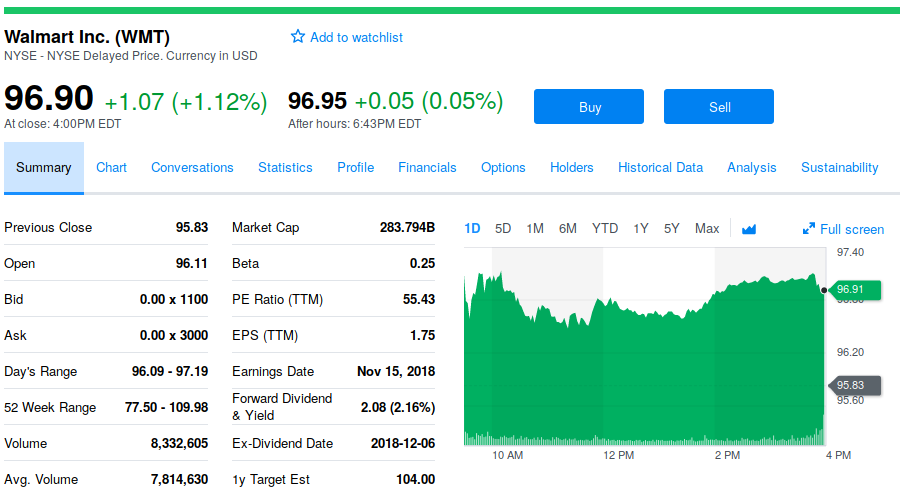
\includegraphics[scale=0.35]{wmt.png}
	\end{center}
	\begin{center}
		Walmart has a beta of \textbf{0.25}
	\end{center}
\end{frame}

%%%%%%%%%%%%%%%%%%  SLIDE  %%%%%%%%%%%%%%%%%%
\begin{frame}{\ftdata{CAPM Beta: Examples}}
	\begin{center}
		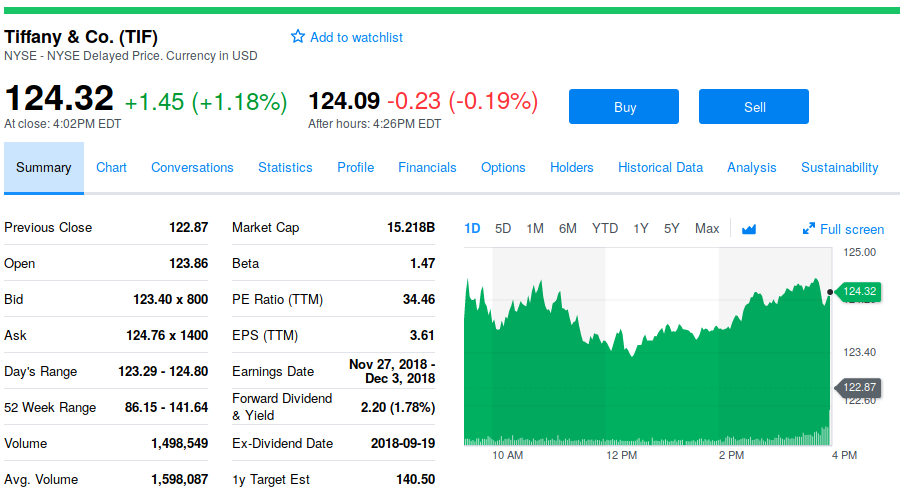
\includegraphics[scale=0.35]{tif.png}
	\end{center}
	\begin{center}
		Tiffany's has a beta of \textbf{1.47}
	\end{center}
\end{frame}

% Variance Decomposition
\begin{frame}{\fttheory{Volaility Decomposition}}
\begin{itemize}
\item The stock's volatility is $\text{SD}[R_{\text{Stock}}]$ 
\item The volatility of a porfolio with the same systematic risk as that of the stock is $\beta_{\text{Stock}}\text{SD}[R_{\text{Market}}]$
\item We say that a fraction 
	\begin{equation}\label{eq:systematic}
		\frac{\beta_{\text{Stock}}\text{SD}[R_{\text{Market}}]}{\text{SD}[R_{\text{Stock}}]}
	\end{equation}
of the stock's volatility is systematic; we say that the remaining fraction is idiosyncratic
\end{itemize}
\end{frame}

% Example
\begin{frame}{\ftexampl{Example}}
	Consider the following data for Cisco (CSCO) and the market
	\begin{center}
		\begin{tabular}{ll}
			$\text{E}[R_{\text{CSCO}}]=0.9961\%$ & $\text{SD}[R_{\text{CSCO}}]=7.09\%$ \\
			$\text{E}[R_{\text{MKT}}]=1.0773\%$ & $\text{SD}[R_{\text{MKT}}]=3.7568\%$ \\
			$\text{Corr}[R_{\text{CSCO}},R_{\text{MKT}}]=0.6339$ & $R_{F}=0.0418\%$
		\end{tabular}
	\end{center}
\begin{enumerate}
	\item What are Cisco's and the market's Sharpe ratios? {\color{blue} .1346, .2756} 
	\item What is Cisco's beta? {\color{blue}1.1963}
	\item What is the market's risk premium? {\color{blue}1.0355\%}
	\item What is Cisco's risk premium? {\color{blue}0.9543\%}
	\item What fraction of Cisco's volatility is systematic? {\color{blue} .6339}
	\item What fraction is idiosyncratic? {\color{blue} .3661}
\end{enumerate}
\end{frame}

% Example
\begin{frame}{\ftexampl{Example}}
	Consider the following data for Caterpillar (CAT) and the market
	\begin{center}
		\begin{tabular}{ll}
			$\text{E}[R_{\text{CAT}}]=1.3424\%$ & $\text{SD}[R_{\text{CAT}}]=8.1365\%$ \\
			$\text{E}[R_{\text{MKT}}]=1.0773\%$ & $\text{SD}[R_{\text{MKT}}]=3.7568\%$ \\
			$\text{Corr}[R_{\text{CAT}},R_{\text{MKT}}]=0.7279$ & $R_{F}=0.0418\%$
		\end{tabular}
	\end{center}
\begin{enumerate}
	\item What are Caterpillar's and the market's Sharpe ratios? 
	\item What is Caterpillar's beta?
	\item What is the market's risk premium? 
	\item What is Caterpillar's risk premium? 
	\item What fraction of Caterpillar's volatility is systematic? 
	\item What fraction is idiosyncratic?
\end{enumerate}
\end{frame}

\begin{frame}{\fttheory{Alpha}}
	\begin{itemize}
	\item The difference between the stock's actual risk premium and the risk premium of a portfolio with the same systematic risk is the alpha:  
	\begin{equation}
		\alpha_{\text{Stock}} = \underbrace{(\text{E}[R_{\text{Stock}}]-R_{F})}_{\text{True Value}}-\underbrace{\beta_{\text{Stock}}\times(\text{E}[R_{\text{Market}}] - R_{F})}_{\text{CAPM}}
	\end{equation}
	\item While one might observe a non-zero alpha in the short-term, it will likely become zero in the long-term
	\end{itemize}
\end{frame}

% Example
\begin{frame}{\ftexampl{Example}}
\begin{enumerate}
	\item What is Cisco's alpha? {\color{blue}-0.2845\%}
	\item What about Caterpillar?
\end{enumerate}
\end{frame}

\begin{frame}
	\begin{center}
		\Huge The Efficient Market Hypothesis 
	\end{center}
\end{frame}

\begin{frame}{\ftheader{The Efficient Market Hypothesis (EMH)}}
	\begin{itemize}
		\item The Efficient Market Hypothesis (EMH) states that prices of securities fully reflect available information about securities
		\item It highlights the difficulties associated with earning abnormal returns using either \textit{fundamental analysis} (predicting returns based on accounting or economic data) or \textit{technical analysis} (predicting returns based on the past history of returns). 
	\end{itemize}
\end{frame}

\begin{frame}{\fttheory{The Random Walk}}
	\begin{itemize}
		\item A stock price follows a \textit{random walk} returns are unpredictable.
		\item Suppose that Apple traded for 266 USD at 12:00 and everyone knew that at the end of the day, it would trade for 270 USD (a risk-free return of 1.5\% in just one afternoon!)
		\item Everyone would start buying. The price would rise to 267 (a return of 1.13\%), to 268 (.75\%), and so on until at 12:01, when the price would be 270 (0\%). 
		\item Put differently, all information (such as the fact that the price will be 270 USD by the end of day) is immediately incorporated into the price
		\item The random walk explains why the stock market does well on days when bad news comes out (e.g. the market expected that unemployment would rise by 1\%, traded stocks at prices reflecting that expectation, and then when unemployment rose by .95\%, stock prices rose).
	\end{itemize}
\end{frame}

\begin{frame}{\fttheory{Forms of the EMH}}
	There are three forms of the hypothesis, depending on how much information it assumes investors have
	\begin{enumerate}
		\item\textbf{Weak Form:} the assertion that stock prices already reflect all information contained in the history of past trading
		\item\textbf{Semi-Strong Form:} the assertion that stock prices already reflect all publicly available information 
		\item\textbf{Strong Form:} the assertion that stock prices already reflect all relevant information including inside information
	\end{enumerate}
\end{frame}

\begin{frame}{\fttheory{Technical Analysis}}
	\begin{itemize}
		\item Technical analysis involves researching recurrent and predictable stock price patterns
		\item It claims that even if prices on average incorporate all publicly information, they deviate in the short-term in predictable ways
		\item It's less about the long-term value of the security and more about its short-term supply and demand
		\item Technical analysts typically attribute these patterns to market psychology. 
		\item History note: technical analysis has its roots in Charles Dow's ``Dow theory'' (Dow, of the Dow Jones Industrial Average and the \text{Wall Street Journal}).
	\end{itemize}
\end{frame}

\begin{frame}{\fttheory{Technical Analysis}}
	\begin{itemize}
		\item Common concepts in technical analysis include \textit{support} (a price below which a stock's price doesn't typically fall) and \textit{resistence} (a price above which a stock's price doesn't typically rise).  
		\item It follows that when a stock's price nears its support, one should buy (it can only go up) and when the price nears its resistence, one should sell (it can only go down).
		\item \textbf{Important Caveat:} one factor identified in research is momentum: specifically the return of a portfolio that goes long stocks that have down well and short stocks that have done poorly. While this certaintly has the flavor of technical analysis, the trading costs of such a strategy are high. 
	\end{itemize}
\end{frame}

\begin{frame}{\ftexampl{Support and Resistence}}
	Consider a stock valued at 10 USD per share. Suppose that the chart shows a support of 9 USD and a resistence of 11 USD and suppose that because of a dividend increase, it is now valued at 15 USD per share. If other traders believe in a resistence level, then as soon as the price nears 11 USD, they will be willing to sell to you for 11 USD. If you buy at 11 USD, then you make a profit of 4 USD, as the present value of the cash flows is 15 USD. In order to realize this profit, the market must either give-up the resistence level or you have to hold the stock long-term and obtain the dividends yourself.
\end{frame}

\begin{frame}{\fttheory{Fundamental Analysis}}
	\begin{itemize}
		\item Fundamental analysis involves research on the determinants of stock value, such as earnings and dividends prospects, expectations for future interest rates, and risk of the firm 
		\item An extreme form of fundamental ``analysis'' involves collecting inside information (e.g. someone on the board tells you on the phone that he will announce a special dividend tomorrow or someone at the Fed tells you that the Fed will lower rates next week). This behavior is typically illegal.
	\end{itemize}
\end{frame}

\begin{frame}{\ftexampl{Fundamental Analysis}}
	Consider our example with support and resistence, but suppose now that the market did not believe in a support or resistence. Fundamental analysis would involve predicting the change in dividend, buying the stock when it traded for 10 USD and selling when it adjusted to 15 USD.  
\end{frame}

\begin{frame}{\fttheory{Technical and Fundamental Analyses: A Summary}}
	\begin{itemize}
		\item Technical analysis can easily be automated and traded \textit{against}. One need only stock price data and a few milliseconds of computer time to identify trading opportunities and submit trade orders.
		\item Example algorithm: if everyone sells at an arbitrary resistence level, then submit a limit buy order at that level; if everyone buys at an arbitrary support level, then submit a limit sell order at that level. You will make money on average. 
		\item Fundamental analysis, in constrast, requires much more work, and the people who do it are compensated for their labor in the form of alpha. 
	\end{itemize}
\end{frame}

\begin{frame}
	\begin{center}
		\Huge Multirfactor Models
	\end{center}
\end{frame}

\begin{frame}{\fttheory{Multifactor Models (APT Part I)}}

	\begin{itemize}
		\item A multifactor model decomposes a security's return into \textit{factors} $f_{1},f_{2},\ldots,f_{N}$:
			\begin{equation}\small
				r_{S}-r_{F}=\alpha+\beta_{1}f_{1}+\beta_{2}f_{2}+\cdots+\beta_{N}f_{N}+\epsilon
			\end{equation}
		\item The CAPM is a 1-factor model with $f_{1}=r_{M}-r_{F}$. 
		\item There are multifactor models for stocks (which we will explore in a moment), bonds, currencies, housing, and other securities. 
		\item In currencies, for example, the two most popular popular factors are ``value'' and ``carry'', each corresponding to the return on a certain portfolio of currencies. 
		\item Again, the APT claims that $\alpha=0$ on average:
			\begin{equation}
				\text{E}[r_{S}-r_{F}]=\beta_{1}\text{E}[f_{1}]+\beta_{2}\text{E}[f_{2}]+\cdots+\beta_{N}\text{E}[f_{N}]
			\end{equation}
	\end{itemize}
\end{frame}

\begin{frame}{\ftdata{Application: Fama-French 3-Factor Model}}
	\begin{itemize}
		\item The Fama-French model is a  multifactor model for stocks. 
		\item It has factors $f_{1}=r_{\text{MKT}}-r_{F}$, $f_{2}=r_{\text{SMB}}$, and $f_{3}=r_{\text{HML}}$.
		\item SMB is a portfolio that goes long (S)mall stocks and short (or (M)inus) (B)ig stocks (as measured by market cap).
		\item Smaller firms outperform bigger firms (3.06\% 1927-2019). 
		\item HML is a portfolio that goes long (H)igh book-to-market stocks and short (or (M)inus) (L)ow book-to-market stocks. 
		\item Two definitions: \textit{value stocks} are stocks with a (H)igh book-to-market ratio, while \textit{growth stocks} are stocks with a (L)ow book-to-market ratio.  
		\item Value stocks outperform growth stocks (4.48\% 1927-2019).
		\item The idea is that smaller stocks and stocks with higher book-to-market are riskier and therefore offer higher returns
		\item \url{https://mba.tuck.dartmouth.edu/pages/faculty/ken.french/data_library.html}
	\end{itemize}
\end{frame}

\end{document}
